\documentclass[dvipdfmx]{beamer}
\usepackage{setspace}
\usepackage{url}

\AtBeginDvi{\special{pdf:tounicode EUC-UCS2}}

\usetheme{metropolis}
\setbeamertemplate{footline}[frame number]\renewcommand{\kanjifamilydefault}{\gtdefault}
\renewcommand{\kanjifamilydefault}{\gtdefault}

\title{プログラミング言語 Scala と Java の紹介}
\author{照井 章}
\institute{筑波大学 数理物質系}
\date{2019年7月16日}

\begin{document}
    
\begin{frame}
    \frametitle{}
    \titlepage

    \begin{center}
        \url{https://github.com/tsukuba-compexer-2019/compexer-2019-tex-intro}
    \end{center}
\end{frame}

\begin{frame}
    \frametitle{この話の内容}
    \large
    \setstretch{1.5}
    \begin{itemize}
        \item プログラミング言語 Scala, Java の生い立ちや特徴など
    \end{itemize}
\end{frame}

\begin{frame}
    \frametitle{Scala とは? (\cite{scala-3}, \cite{scala-3-jp}, \cite{scala})}

    \begin{block}{プログラミング言語}
        \begin{itemize}
            \item オブジェクト指向プログラミング言語と関数型プログラミング言語の特徴を持つ
            \item Javaのライブラリが利用可能
            \item コンパイルするとJava仮想マシン上で動作する
        \end{itemize}
    \end{block}
\end{frame}

\begin{frame}
    \frametitle{Scala の設計者}
    Martin Odersky (1958--)
    \begin{itemize}
        \item コンピュータ科学者
        \item スイス連邦工科大学ローザンヌ校 教授\\
        Professor, \'Ecole Polytechnique F\'ed\'erale de Lausanne (EPFL)
    \end{itemize}
    \begin{center}
        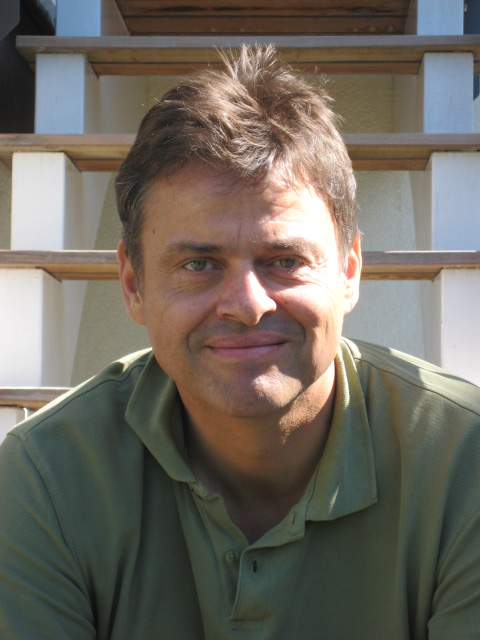
\includegraphics[scale=0.5]{Martin.jpeg}\\
        (From his homepage \cite{odersky})
    \end{center}
\end{frame}

\begin{frame}
    \frametitle{Scalaの歴史 \cite{scala-history}}
    \large
    \begin{itemize}
        \item 大学院時代(スイス連邦工科大学チューリッヒ校): Niklaus Wirth(ニクラウス ヴィルト)教授のもとで学び、数々のコンパイラのプロジェクトに参加し、関数型プログラミングに熱中する
        \item 1990年代後半:JavaコンパイラおよびJava言語仕様(総称型)の開発に携わる
        \item 2001年: Scalaの開発を開始
        \item Scalaの導入例: Twitter, ドワンゴ(ニコニコ生放送)など (\cite{scala-users-jp}, \cite{scala-old})
    \end{itemize}
\end{frame}

\begin{frame}
    \frametitle{Java とは? (\cite{java-bible}, \cite{oracle-java}, \cite{java-magazine})}

    \begin{block}{主に2つの意味}
        \begin{enumerate}
         \item プログラミング言語
         \item Java言語を中心とした情報処理環境
        \end{enumerate}
    \end{block}

    \begin{block}{プログラミング言語の特徴}
        \begin{itemize}
            \item オブジェクト指向プログラミング言語
            \item 「一度書けばどこでも動く』(家電機器、乗用車、パソコン、サーバ\dots)
            \item コンパイルするとJava仮想マシン上で動作する
            \item 並列処理やネットワークとの連携を前提にした設計
        \end{itemize}
    \end{block}
\end{frame}

\begin{frame}
    \frametitle{Java の設計者}
    James Gosling (1955--)
    \begin{itemize}
        \item ソフトウェア技術者
        \item 元サン・マイクロシステムズ (Sun Microsystems) フェロー
    \end{itemize}
    \begin{center}
        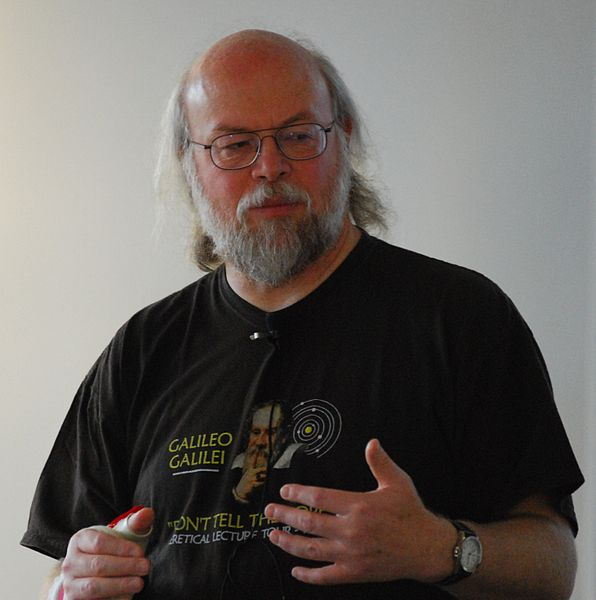
\includegraphics[scale=0.2]{596px-James_Gosling_2008.jpg}\\
        (Photo: Peter Campbell, CC BY-SA 4.0 \cite{campbell})
    \end{center}
\end{frame}


\begin{frame}
    \frametitle{Java(とSun Microsystems)の歴史 \cite{java-history}}
    \large
    \begin{itemize}
        \only<1>{
        \item Sunは1980年代後半から1990年代前半にかけてUNIXワークステーションの業界に君臨
        \item 1990年代中盤から始まったインターネットの普及を背景に、家電製品からサーバまで様々な機器で動く言語を設計し、普及する
        \begin{itemize}
            \item パソコンのアプリケーション: Java SE (Java Platform, Standard Edition)
            \item 企業の情報システム: Java EE (Java Platform, Enterprise Edition )
            \item 組込機器: Java ME (Java Platform, Micro Edition)
        \end{itemize}
        }
        \only<2>{
        \item 21世紀に入り、SunはIntelをはじめとする安価なCPUによるLinuxサーバの普及などに追い抜かれる
        \item Sunは2010年にソフトウェア企業のオラクル (Oracle) によって買収され、Javaの所有権もOracleに移る
        \item 現在はOracleの製品として開発が継続されている
        }
    \end{itemize}
\end{frame}


\begin{frame}[allowframebreaks]
    \frametitle{参考文献}
    \begin{thebibliography}{99}
        \bibitem{java-bible}
        ケン・アーノルド, ジェームズ・ゴスリン, デビッド・ホームズ 著, 柴田芳樹 訳. 
        プログラミング言語Java 第4版. 東京電機大学出版局, 2014.

        \bibitem{campbell} Peter Campbell. James Gosling. 2008, \url{https://commons.wikimedia.org/wiki/File:James_Gosling_2008.jpg} (参照 2019-07-15).

        \bibitem{java-history}
        Linuxアカデミー. エンジニアリングの入り口: Javaの歴史を一通りなぞってみる. 2019. \url{https://eng-entrance.com/java-history} (参照 2019-07-15).

        \bibitem{odersky} Martin Odersky. \url{https://lampwww.epfl.ch/~odersky/} (参照 2019-07-15).

        \bibitem{scala-3} Martin Odersky, Lex Spoon, Bill Venners. Programming in Scala, Third Edition. Artima, 2016, 859p.

        \bibitem{scala-3-jp}
        Martin Odersky, Lex Spoon, Bill Venner 著, 長尾高弘 訳, 羽生田栄一, 水島宏太 監訳. Scalaスケーラブルプログラミング第3版. インプレスブックス, 2016, 720p.

        \bibitem{scala-history} Martin Odersky. A Brief History of Scala, Artima.com weblogs, 9 June 2006. \url{https://www.artima.com/weblogs/viewpost.jsp?thread=163733} (参照 2019-07-15).

        \bibitem{oracle-java} Oracle Corporation. Java. \url{https://www.java.com/ja/} (参照 2019-07-15).

        \bibitem{java-magazine} Oracle Corporation. Java Magazine(日本版). \url{https://www.oracle.com/technetwork/jp/java/index.html} (参照 2019-07-15).

        \bibitem{scala-users-jp} 日本Scalaユーザー会. 採用事例(国内). \url{http://jp.scala-users.org/scala-cases-in-japan.html} (参照 2019-07-15).

        \bibitem{scala} The Scala Programming Language. \url{https://https://www.scala-lang.org/} (参照 2019-07-15).

        \bibitem{scala-old}
        Scala in the Enterprise. \url{https://www.scala-lang.org/old/node/1658} (参照 2019-07-15).

        
    \end{thebibliography}    
\end{frame}

\end{document}